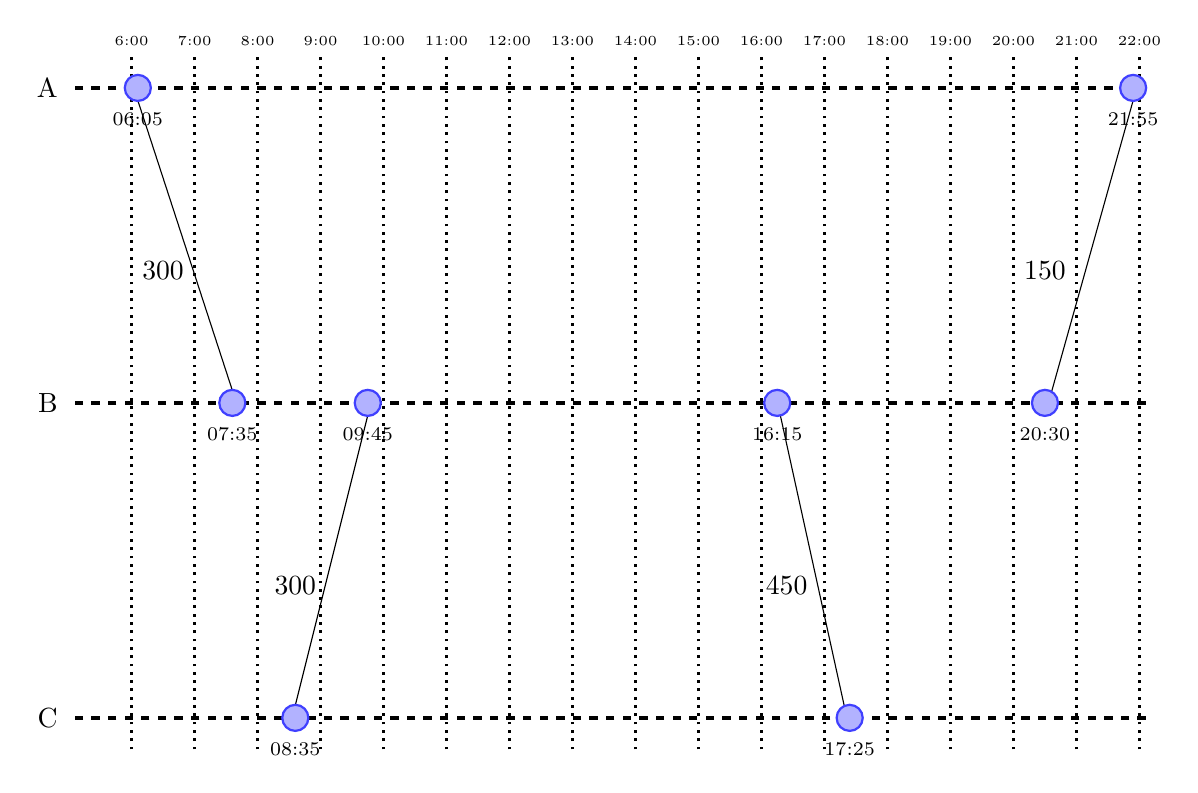
\begin{tikzpicture}[scale=.08]
  \tikzstyle{mynode}=[circle, thick, draw=blue!75, fill=blue!30,
    minimum size=3mm]
  \foreach \t in {6, 7, ..., 22} {
    \draw[line width=1pt, dotted] ({10*(\t-5)}, 0) -- ({10*(\t-5)}, 110)
      node[above, font=\tiny] {\t:00} ;
  }
  \draw[line width=1.2pt, dashed] (171, 105) -- (0, 105) node[left, font=\normalsize] {A};
  \draw[line width=1.2pt, dashed] (171, 55) -- (0, 55) node[left, font=\normalsize] {B};
  \draw[line width=1.2pt, dashed] (171, 5) -- (0, 5) node[left, font=\normalsize] {C};
  \draw[-] (11, 103) -- (26, 57);
  \draw[-] (155, 53) -- (169, 103);
  \draw[-] (113, 53) -- (124, 3);
  \draw[-] (36, 7) -- (47.5, 53);
  \node[mynode] (A-06:05) at (11, 105) {};
  \node[font=\normalsize] at (15, 76) {300};
  \node[font=\scriptsize] at (11, 100) {06:05};
  \node[mynode] (B-07:35) at (26, 55) {};
  \node[font=\scriptsize] at (26, 50) {07:35};
  \node[mynode] (C-08:35) at (36, 5) {};
  \node[font=\normalsize] at (36, 26) {300};
  \node[font=\scriptsize] at (36, 0) {08:35};
  \node[mynode] (B-09:45) at (47.5, 55) {};
  \node[font=\scriptsize] at (47.5, 50) {09:45};
  \node[mynode] (B-16:15) at (112.5, 55) {};
  \node[font=\normalsize] at (114, 26) {450};
  \node[font=\scriptsize] at (112.5, 50) {16:15};
  \node[mynode] (C-17:25) at (124, 5) {};
  \node[font=\scriptsize] at (124, 0) {17:25};
  \node[mynode] (B-20:30) at (155, 55) {};
  \node[font=\normalsize] at (155, 76) {150};
  \node[font=\scriptsize] at (155, 50) {20:30};
  \node[mynode] (A-21:55) at (169, 105) {};
  \node[font=\scriptsize] at (169, 100) {21:55};
\end{tikzpicture}

